\section{MediaSense}
MediaSense is a middleware platform that supports the concept Internet of Things, it was developed to provide a scalable platform with a real time access to context information \cite{Kanter539187}. With all sensors around us in our everyday life applications can collect and share context information to each other. MediaSense provides this functionality and enabling support for applications and services to share and collect context information from such as sensors in specific state. The platform is developed so the complexity is low which is enabling users to focus on developing application and services without caring about how context information is shared and how the layers in the platform is interacting with each other \cite{Walters413794}. 

\subsection{Networking Paradigm}
MediaSense is using a decentralized network also called a peer-to-peer overlay to connect nodes in the network. Context information is then persisted in the network and applications can share and collect information in real time from other nodes in the network. A node in the network can act as both a producer and consumer at the same time which enabling bidirectional access to context information. The decentralized network consists of an overlay that use a P-Grid \cite{aberer2003p} structure as its underlying peer-to-peer technique.

The overlay in MediaSense was first implemented with a Dynamic-Hash-Table. In \cite{Walters413794} the authors discovered that the overlay structure needed to be improved and they chose to use a P-Grid structure for the overlay. Because a lot of users with a lot of applications and services is going to share context information it is important to have a overlay structure that is reliable and can handle the scalability \cite{aberer2003p}. One of the benefits with P-Grid is that it is self organizing. This makes it possible to handle the scalability well.

\subsection{Applications}
MediaSense is written in the programming language Java. MediaSense provides an API that can be used to communicate with the platform. The communication from one platform on a device to another device running the platform is done with messages. The API provides methods for registering new context information and find nodes holding specific context information. Each node attached to the network generates information on a continual basis that is accessed and used by other nodes wishing to do so. In order to do this each node registers itself with a UCI (Universal Context Identifier). The UCI is stored in the distributed network and other nodes can resolve this and get the address where some required information is stored. When a MediaSense instance gets a message a the dissemination layer in MediaSense  handles this message and sending it to the application. The dissemination layer is acting like a router and delivers the messages to the right place. Applications have a method that is handling messages that is routed from the dissemination layer. 

\begin{figure}[H]
	\centering
    	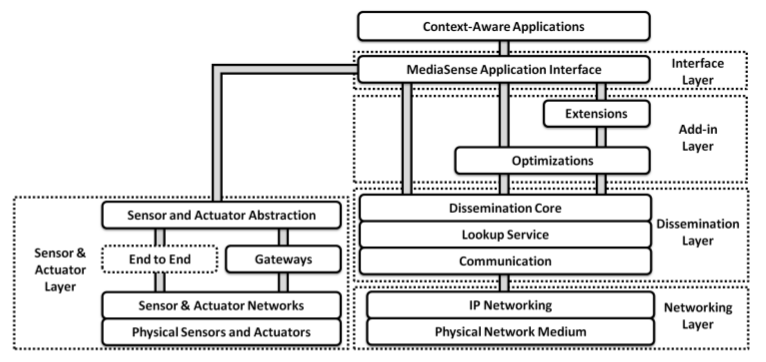
\includegraphics[scale=0.50]{part_2/mediasense/ms_arch.png}
		\caption{MediaSense component architecture \cite{Kanter539187} }
\end{figure}

\subsection{Messages}
As mentioned MediaSense communicates with messages. Applications can register what messages they are interested in. When the platform gets a new message from another node in the network the message will be handled by the dissemination core which then will send the message to the application on the platform that is interested in this kind of message. There are several types of messages. The table shows the basic messages that are available for registering and retrieving information. 

\begin{center}
    \begin{tabular}{ | l | p{12cm} |}
    \hline
    Message name 		& 		Description \\ \hline
	REGISTER UCI 		& 		Registers a UCI along with the node which is responsible for it. \\ \hline
	RESOLVE UCI 		& 		Resolves a UCI to the node which is responsible for it. \\ \hline
	GET 				& 		Fetches the current context value from the node responsible for a UCI. The reply is sent using a NOTIFY. \\ \hline
	SET 				& 		Changes the current status of an actuator in an end point. \\ \hline
	SUBSCRIBE 			& 		Makes a subscription request to the node responsible for a UCI, The node then sends a NOTIFY message containing the current context value, either at regular intervals or when the value changes. \\ \hline
	NOTIFY 				& 		Notifies an interested node of the current context value associated with a specified UCI. \\ \hline
	TRANSFER 			& 		Requests the manager of a resource to transfer responsibility to another node. This might be full responsibility or partial, where the requester re-creates a copy of the resource permitting improved real time performance. \\ \hline
    \end{tabular}
\end{center}

\subsection{Instances of MediaSense}
When an application is run that wishes to use the MediaSense platform, the application must initialize and use its own instance of MediaSense. For example if a user have an application, Application 1 this application need an instance of MediaSense to access context information. If the user have an application, Application 2 running on the same device this application also need its own MediaSense instance to access context information. Every instance of MediaSense is seen as one node, so if we have two instances of the platform on one device this device is acting as two nodes in the network. This is misleading because one node in the network should be one device and not one application.

\begin{figure}[t]
	\centering
    	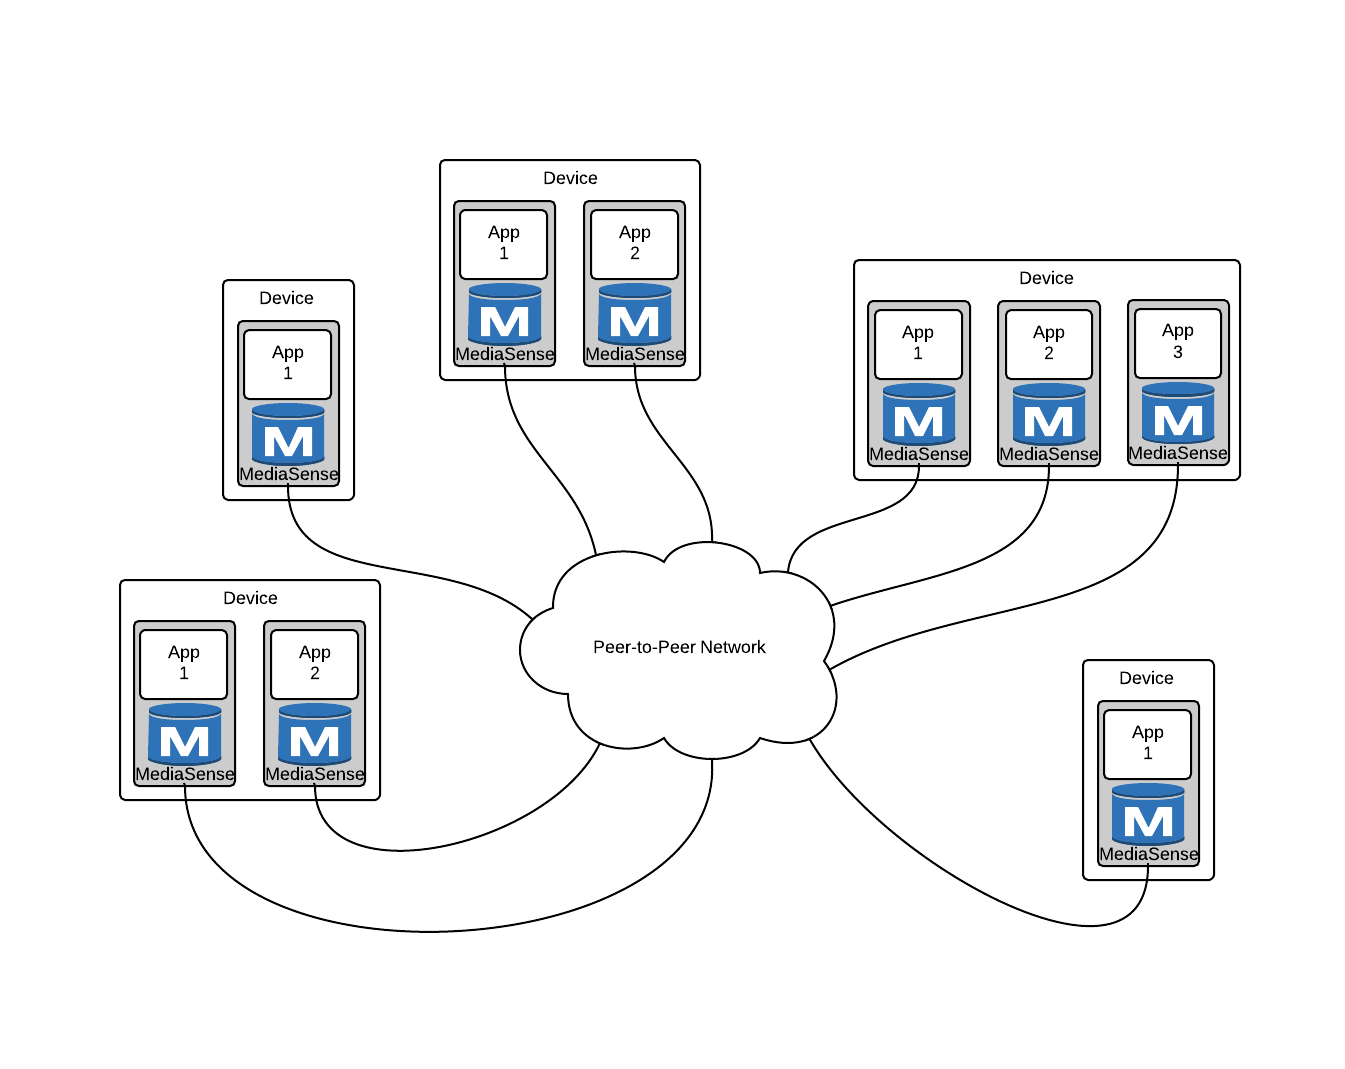
\includegraphics[scale=0.25]{part_2/mediasense/several_nodes_on_one_device.png}
		\caption{Figure showing how the instances of MediaSense is connected to the network} 
\end{figure}

Each instance of MediaSense requires that a new port be opened so the network layer can communicate with other nodes in the network. This means that if the user is behind a NAT or a firewall the user needs to open up new ports for every instance of MediaSense. The amount of open ports is equal to the amount of applications running on a device. This can be seen as a security issue. With more port open the device that is running the platform is more vulnerable.
Not only that the device will be more vulnerable, when a user need several instances of MediaSense and every instance need its own port the network usage will increase. This can affect the battery time of a ubiquitous device in a negative way.

One more thing to consider with an application invoked platform is that the memory usage will increase. Every instance of MediaSense need to use a specific amount of memory. If the platform is running on a ubiquitous device this will limit the number of applications running on the device, because of the several instances of MediaSense.

To make MediaSense more efficient we need to reduce the resource footprint, without losing  the functionality. This can be done in several ways. One way is to change the overlay architecture and use a centralized approach for sharing and collecting context information. This solution will make every application connecting to a centralized server or to use a internet portal, for example RESTful API to access the data. The problem with this is that they are centralized and therefore not well scalable and we will lose the functionality of P-Grid. They are also dependent on DNS which means that applications expect that the centralized server are always available. As mentioned before centralized solutions are more vulnerable and can be attacked with Denial-of-service attacks. If the centralized server is having DNS errors the context information can not be accessed and shared to other applications and the applications is usable. Examples of Internet of thing services using this architecture is SenseWeb and Sensei. This two examples is using centralized web-services for sharing context information which makes them having the mentioned issues and are therefore not a good solution for an Internet of things service.